\documentclass[12pt,oneside]{sotsuken_paper}
\usepackage{amsmath}
\usepackage{flow}
\usepackage[dvipdfmx]{color}
\usepackage[dvipdfmx]{graphicx}
%\usepackage[dviout]{graphicx}

% タイトル
\title{音声認識を用いて接客をするロボットの開発}
\author{金沢工業高等専門学校 澤田茂人}

\begin{document}
% 行間
\setlength{\baselineskip}{9truemm}

%文字間
\kanjiskip=.53zw plus 3pt minus 3pt
\xkanjiskip=.53zw plus 3pt minus 3pt

% 目次
\tableofcontents
%\newpage

% 本文

\chapter{序論}
\section{研究の背景}
近年ソフトバンク社がPepperを開発した.また,長崎県に存在するテーマパーク「ハウステンボス」で宿泊する際に利用すると考えられる「変なホテル」の受付には女性タイプと恐竜タイプの接客ロボットや話しかけることで照明のオンオフを行ってくれるロボットなどが配備されている.本研究は飲食店にて接客業務での人件費削減を行うため,ロボットを制作してほしいという要望があった.そこで音声でのやりとりをするためのシステムを開発する必要があると考え,本研究を開始した.飲食店で注文を取るロボットに使用した音声を認識させるシステムについて今から述べていく.図\ref{fig:hospitality-robot}にpepper,図\ref{fig:huistenbosch_human}にホテルに存在する女性タイプの接客ロボット,図\ref{fig:huistenbosch_dinosaur}に恐竜タイプの接客ロボットの外観を示す.


\begin{figure}[htbp]
\begin{center}
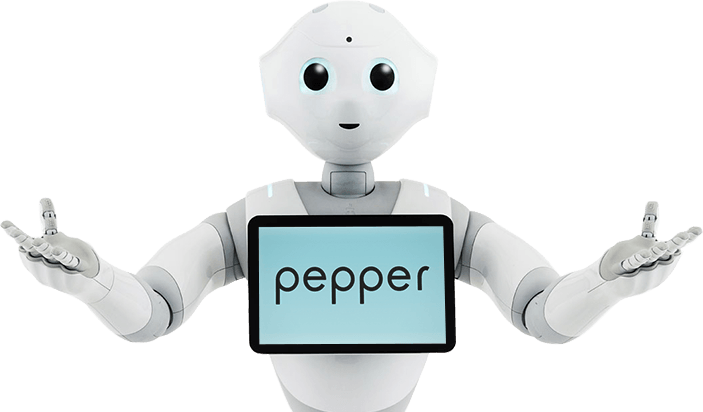
\includegraphics[width=120mm]{img/pepper.png}
\caption{pepper}
\label{fig:hospitality-robot}
\end{center}
\end{figure}


\begin{figure}[htbp]
\begin{center}
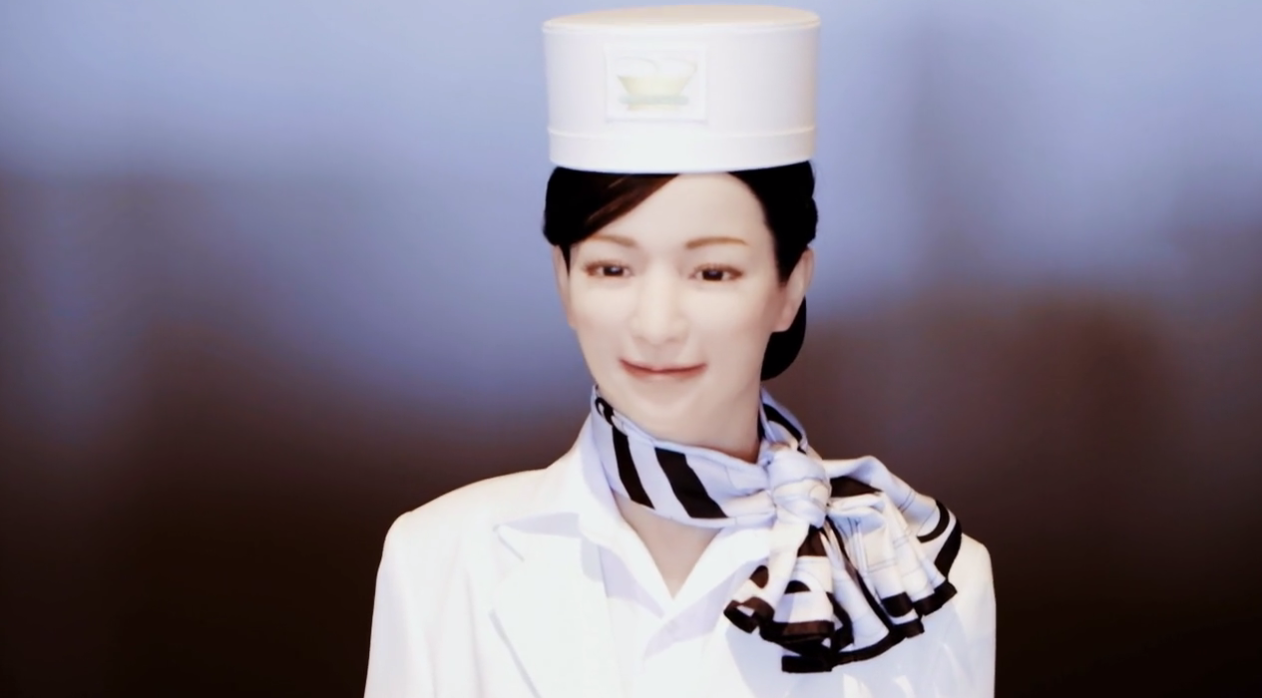
\includegraphics[width=120mm]{img/huistenbosch_human.png}
\caption{女性タイプの接客ロボット}
\label{fig:huistenbosch_human}
\end{center}
\end{figure}


\begin{figure}[htbp]
\begin{center}
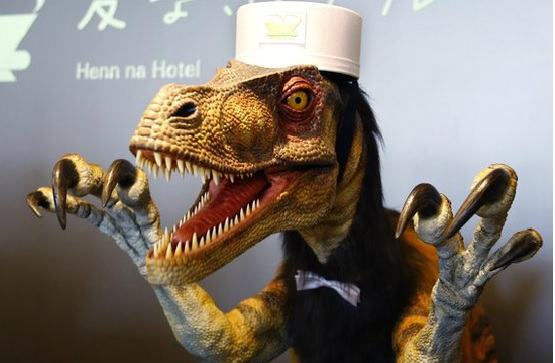
\includegraphics[width=120mm]{img/huistenbosch_dinosaur.jpg}
\caption{恐竜タイプの接客ロボット}
\label{fig:huistenbosch_dinosaur}
\end{center}
\end{figure}


\section{研究の目的}
飲食店にてPCを実装したロボットに音声認識をするためJulius,Open-JTalk,認識すべき単語,マイクを準備し飲食店で禁煙か喫煙かの判断や「あちらの席へどうぞ」「こちらの席へどうぞ」のようなレベルの案内をすることを目的とする.図\ref{fig:yousu}に音声認識をしようとしたときのイメージ図を示す.
\begin{figure}[htbp]
\begin{center}
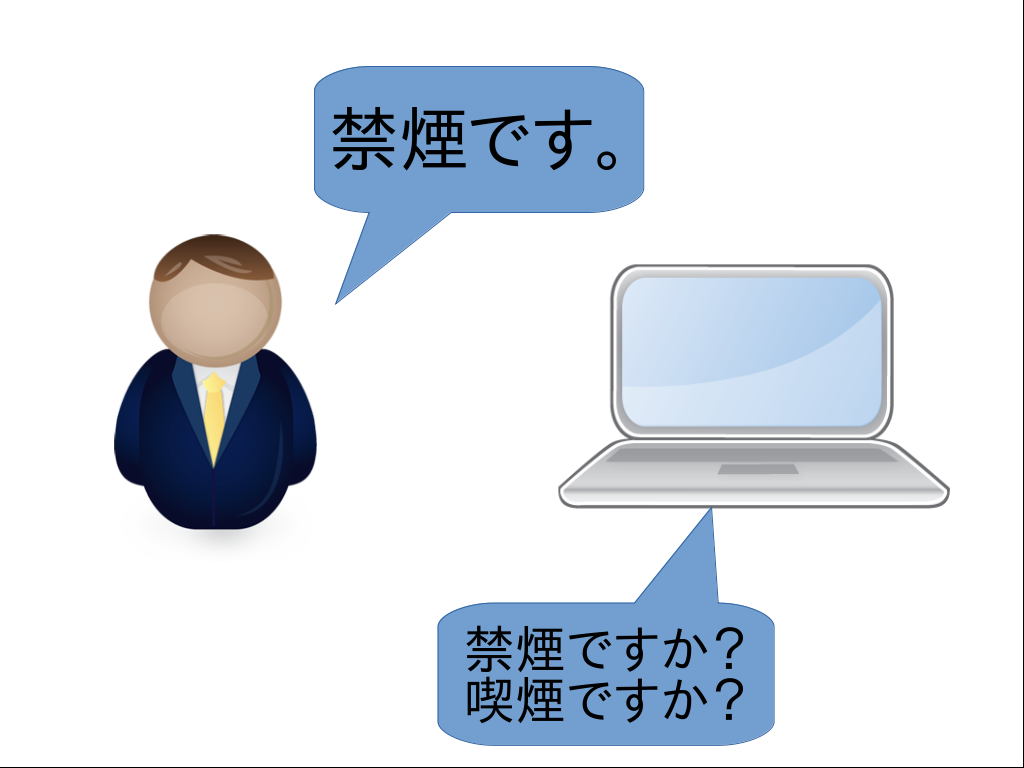
\includegraphics[width=120mm]{img/Image.png}
\caption{様子}
\label{fig:yousu}
\end{center}
\end{figure}
\section{論文の構成}
この論文は以下のように構成されている.


1章では,音や音声について,研究背景について述べた.


2章では,本研究に使用する,音声を認識するための道具及び発生する音声について述べる.


3章では,本研究のために構築した検討用のシステムについて述べる.


4章では,前章で述べた検討用のシステムを使用して行った実験について述べる.


5章では,本研究のまとめや今後の課題について述べる.
\chapter{飲食店での接客について}
\subsection{接客の業務内容}
お客さまから注文を取り,出来上がった料理や飲み物を運び,空いた皿の片付け,レジ業務を行うのが主な仕事である.その接客の業務内容の流れをフロチャートを図\ref{fig:customer-service}に示す.

\begin{figure}[htbp]
%\begin{center}
%\documentstyle
\scriptsize
\setiftext{yes}{no}
\STRUCT{開始}{}{%
    \ACTION{\centering{お出迎えする.}}%
    \ACTION{人数の確認.}%
        \CASE{禁煙喫煙の確認.}{%
        \WHEN{禁煙の場合}{%
            \ACTION{\centering{あちらの席へどうぞ.}}%
        }%
        \WHEN{喫煙の場合}{%
            \ACTION{\centering{こちらの席へどうぞ.}}%
        }%
        \WHEN{5人以上の客でなおかつ禁煙の場合}{%
            \ACTION{\centering{「ただいま席をお作りしますので少しお待ちください.」}}%
        }%
    }%
    \ENDCASE%
    \ACTION{\centering{オーダーを取る.}}%
    \ACTION{\centering{料理を出す.}}%
    \ACTION{\centering{レジで会計を行う.}}%
}%
\caption{接客方法の流れ}
\label{fig:customer-service}%
\normalsize
%\end{center}
\end{figure}


\subsection{研究として検討する接客の業務内容}
接客の仕事内容をフローチャートとして挙げたが今回,接客をするロボットの開発を行うにあたり,店の入口付近で客がタバコを吸うかどうかの判断や「あちらの席へどうぞ」「こちらの席へどうぞ」の案内をすることが研究として検討する接客の業務内容となる.


\section{声とは}
声とは空気の振動であり波である.つまりsinカーブで表すことができ,人間が声として発する「あ」という音一つから「卒業研究」のような単語,「私の職業は学生であるため勉強をすることが仕事である.」と言った文章を声で発している限りsinカーブで表すことができる.人間の声をマイクに入れてそのデータをの周波数成分を明らかにするためには特別な手段を用いる必要がある.それは音声にフーリエ変換を掛けることである.


\subsection{フーリエ変換とは}
まず,フーリエ変換は式\ref{eq:fu-rie}で示すことが出来る.式\ref{eq:fu-rie}より関数f(t)と$e^{-jωt}$を掛けあわせて積分することにより2つの関数が似ていれば絶対値が大きな値,似ていなければ小さな値を取りますので関数f(t)は時間の関数でもあるためオシロスコープでも確認することが可能である.また,回転の成分としてスペクトラムアナライザーでも確認することが出来る.[1]

\setcounter{equation}{0}
\begin{equation}
 F(ω)=\int^{\infty}_{-\infty} f(t)e^{-jωt}dt=0
\end{equation}
\label{eq:fu-rie}

\subsection{高速フーリエ変換とは}
前述の通り声は空気の振動のため実際に視覚的に見ようとした場合,特別な手段を用いなければならない.ここではマイクを使い視覚的に表示することで音声の波形を見ることができると考え,実際にaudacityという音声の編集ソフトを使用して音の波形を視覚的に確認することに成功した.ここで,音の波形を高速フーリエ変換にかける.高速フーリエ変換は英語でFast Fourier Transformと呼ばれていることから頭文字を取ってFFTとも呼ばれている(以下FFTとする).前述に示したフーリエ変換に各音専用の係数をかけることでFFTを行うことができる.図\ref{fig:voice-a}に「あ」の音声波形,図\ref{fig:voice-i}に「い」の音声波形,図\ref{fig:voice-u}に「う」の音声波形,図\ref{fig:voice-e}に「え」の音声波形,図\ref{fig:voice-o}に「お」の音声波形,図\ref{fig:a_fft}に「あ」にFFTをかけた波形,図\ref{fig:i_fft}に「い」にFFTをかけた波形,図\ref{fig:u_fft}に「う」にFFTをかけた波形,図\ref{fig:e_fft}に「え」にFFTをかけた波形,図\ref{fig:o_fft}に「お」にFFTをかけた波形を示す.


\begin{figure}[htbp]
\begin{center}
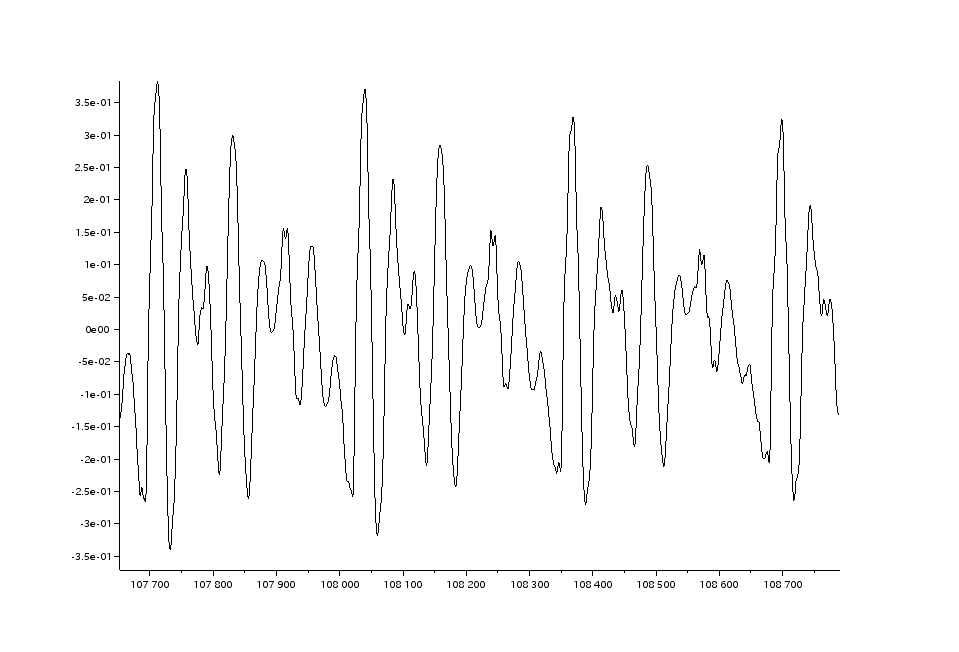
\includegraphics[width=120mm]{img/a.png}
\caption{「あ」の音声波形}
\label{fig:voice-a}
\end{center}
\end{figure}


\begin{figure}[htbp]
\begin{center}
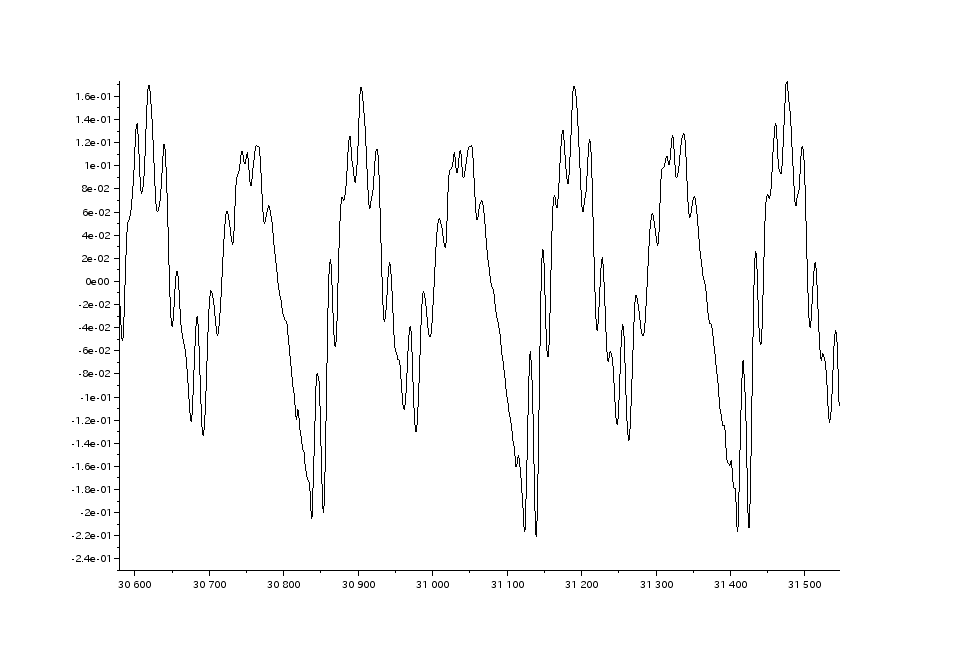
\includegraphics[width=120mm]{img/i.png}
\caption{「い」の音声波形}
\label{fig:voice-i}
\end{center}
\end{figure}


\begin{figure}[htbp]
\begin{center}
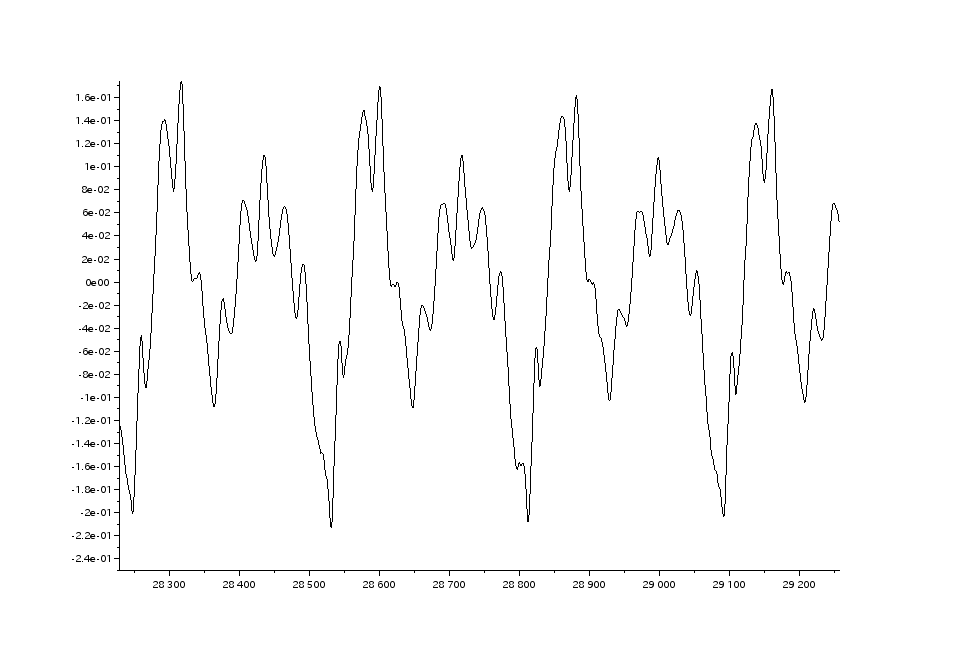
\includegraphics[width=120mm]{img/u.png}
\caption{「う」の音声波形}
\label{fig:voice-u}
\end{center}
\end{figure}


\begin{figure}[htbp]
\begin{center}
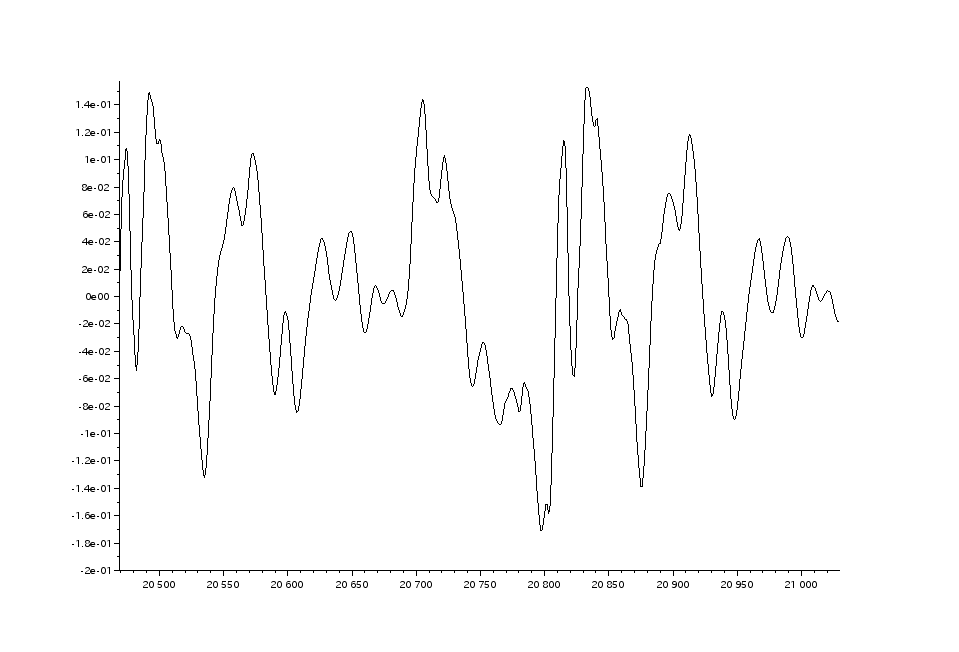
\includegraphics[width=120mm]{img/e.png}
\caption{「え」の音声波形}
\label{fig:voice-e}
\end{center}
\end{figure}


\begin{figure}[htbp]
\begin{center}
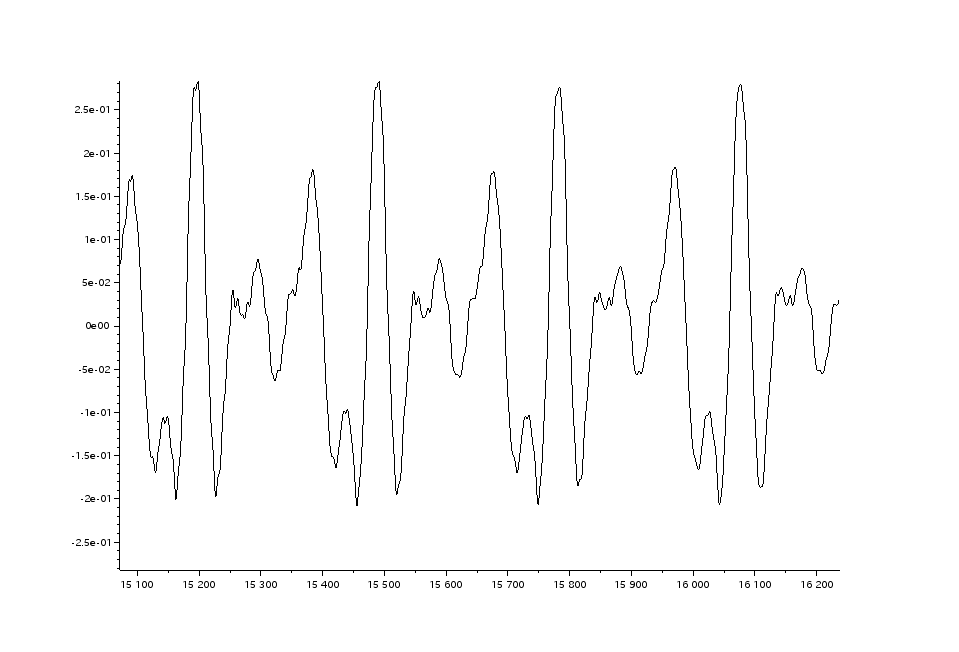
\includegraphics[width=120mm]{img/o.png}
\caption{「お」の音声波形}
\label{fig:voice-o}
\end{center}
\end{figure}


\begin{figure}[htbp]
\begin{center}
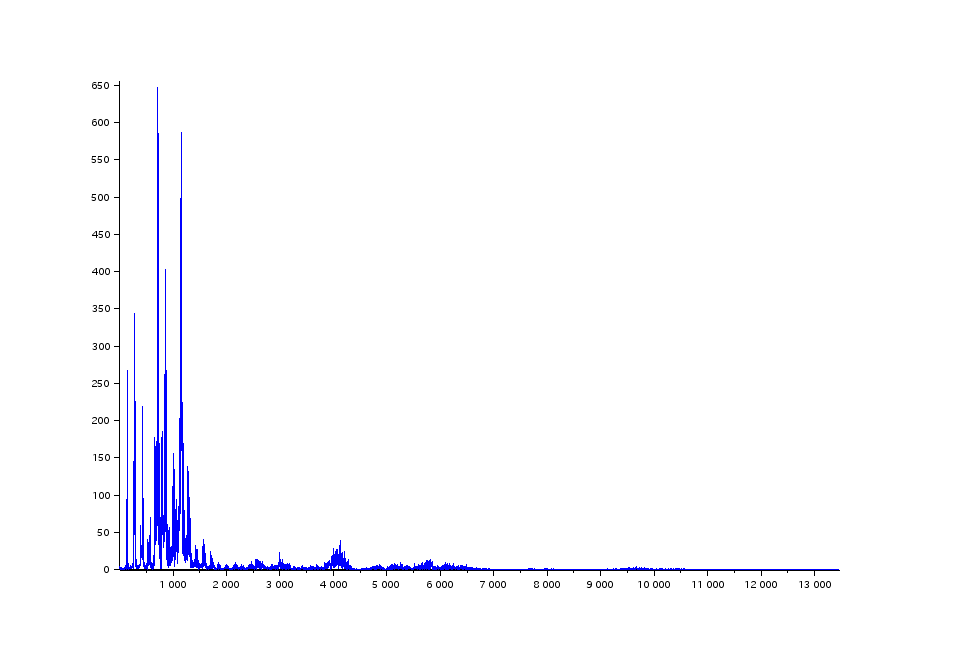
\includegraphics[width=120mm]{img/a_fft.png}
\caption{fftを掛けた「あ」の波形}
\label{fig:a_fft}
\end{center}
\end{figure}


\begin{figure}[htbp]
\begin{center}
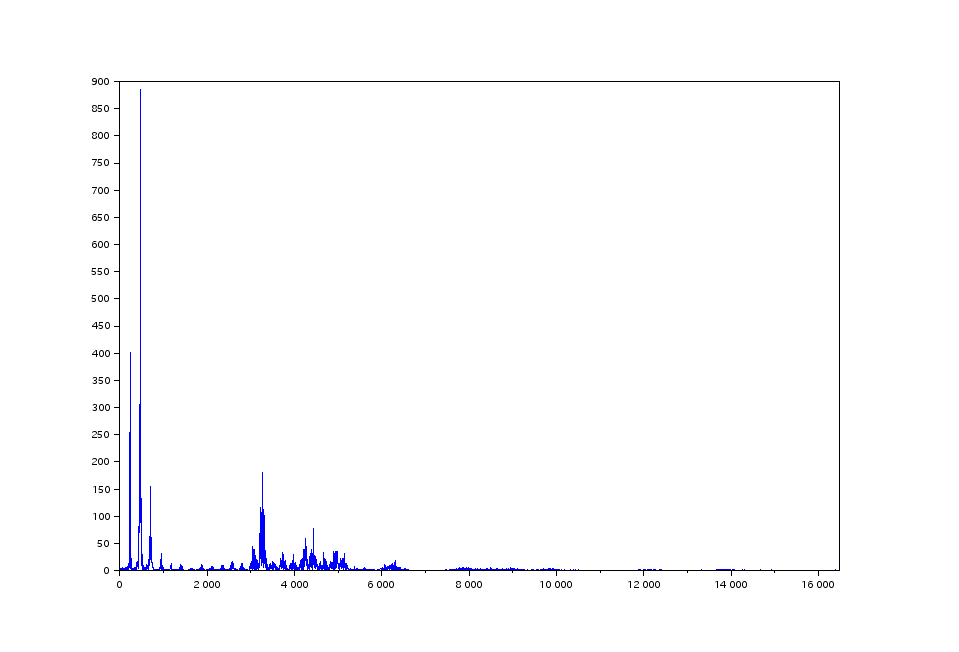
\includegraphics[width=120mm]{img/i_fft.png}
\caption{fftを掛けた「い」の波形}
\label{fig:i_fft}
\end{center}
\end{figure}


\begin{figure}[htbp]
\begin{center}
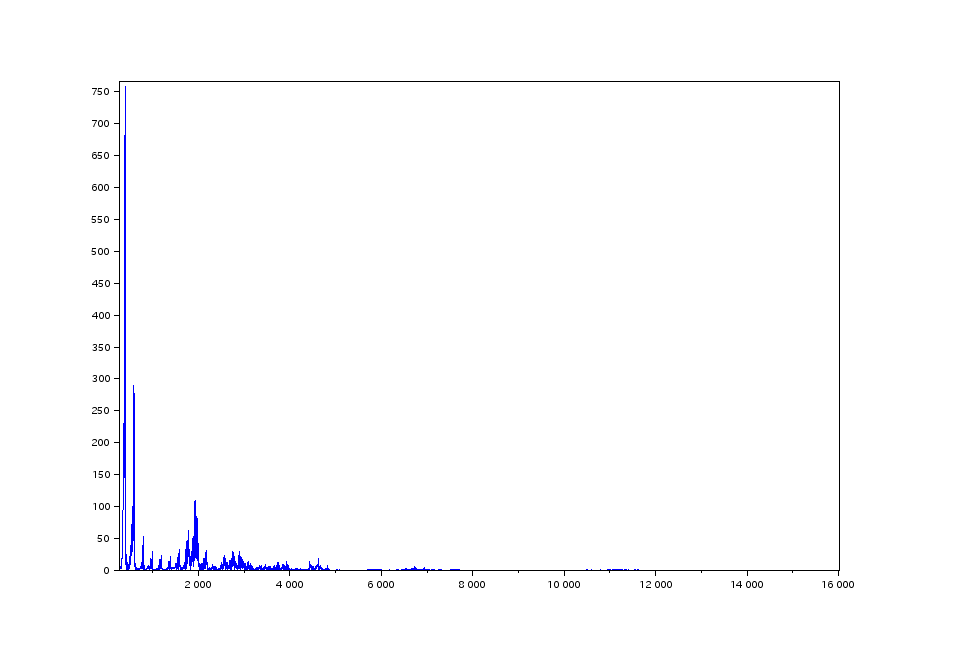
\includegraphics[width=120mm]{img/u_fft.png}
\caption{fftを掛けた「う」の波形}
\label{fig:u_fft}
\end{center}
\end{figure}


\begin{figure}[htbp]
\begin{center}
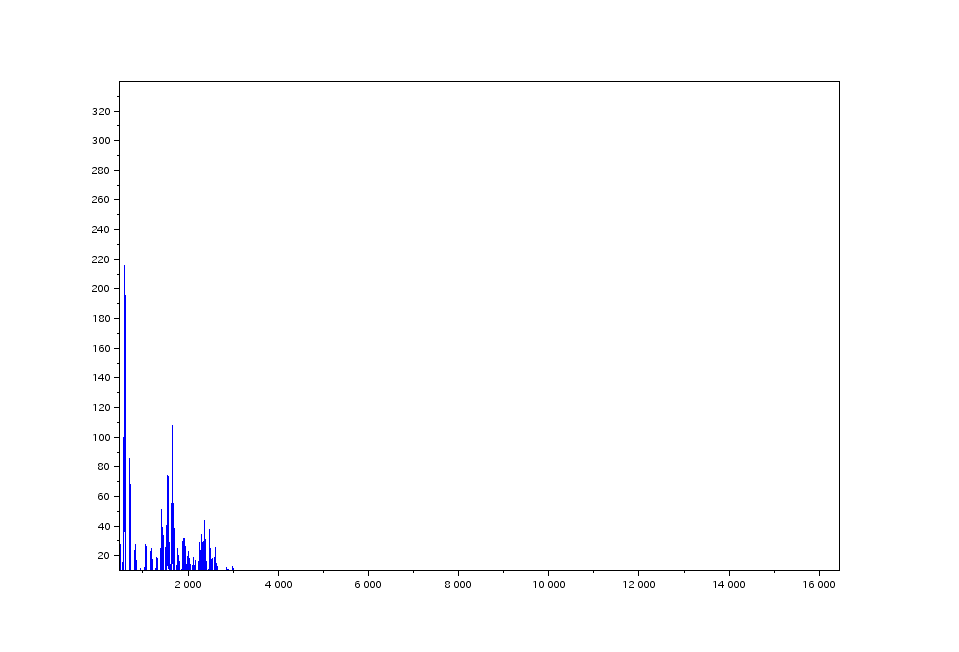
\includegraphics[width=120mm]{img/e_fft.png}
\caption{fftを掛けた「え」の波形}
\label{fig:e_fft}
\end{center}
\end{figure}


\begin{figure}[htbp]
\begin{center}
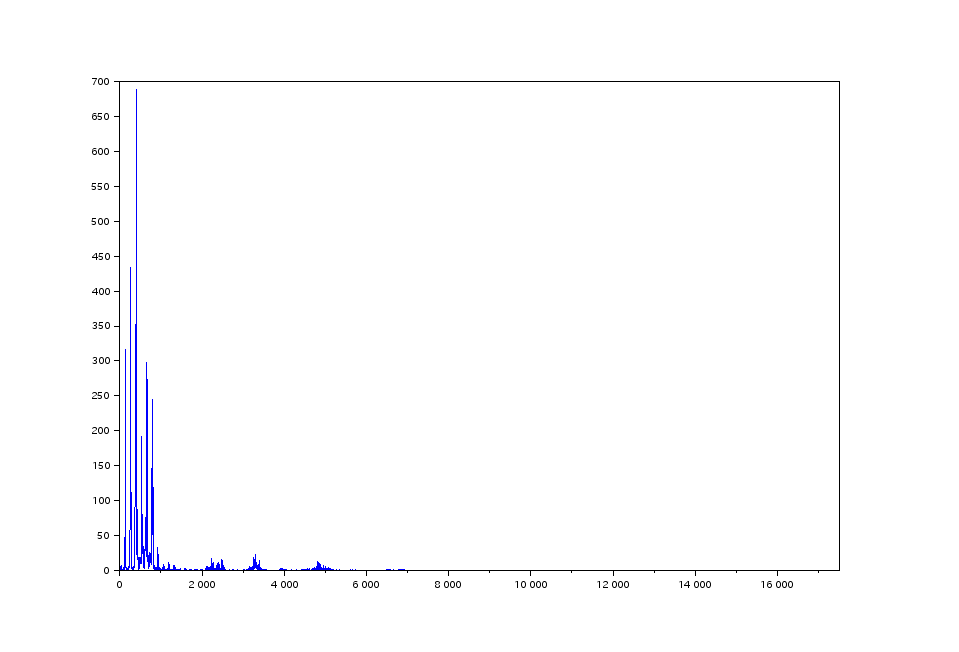
\includegraphics[width=120mm]{img/o_fft.png}
\caption{fftを掛けた「お」の波形}
\label{fig:o_fft}
\end{center}
\end{figure}


\section{各社音声認識用ソフトの調査}
音声によるロボットを制作するにあたり,まずは音声を認識することが必要条件である.そのため,音声を認識するプログラムを作成し使用することが考えられるのだが時間的コストがかかることが予想された.そのため音声を認識するためのソフトを調査した.調査した結果,Julius,ドラゴンスピーチ,docomo音声認識API,Ami Voice,Google Speech APIの5つが候補として挙がった.Juliusを除いた音声認識ソフトは無料のソフトを選択した場合使用期限があり,有料版を選んだ場合金銭的コストがかかるため本研究ではlinuxでも使用でき無料かつ使用期間の制限がないJuliusを選択した.表\ref{tab:speechrecog}に音声認識一覧を示す.また,本研究で使用することとした音声認識ソフトJuliusのアイコンを図\ref{fig:Julius}に示す.

\begin{table}[htb]
\begin{center}
\caption{音声認識一覧}
\begin{tabular}{|c|c|c|c|}\hline
ソフト名&無料である&使用期限がない&認識率 \\ \hline
Julius&○&○&90\%以上 \\ \hline
ドラゴンスピーチ & $\times$ & $\times$ & 不明 \\ \hline
docomo音声認識API&$\times$&$\times$&不明\\\hline
Ami Voice&$\times$&$\times$&不明\\\hline
Google Speech API&$\times$&$\times$&不明\\\hline
\end{tabular}
\label{tab:speechrecog}
\end{center}
\end{table}


\begin{figure}[htbp]
\begin{center}

\includegraphics[width=120mm]{img/Julius.png}
\caption{Julius}
\label{fig:Julius}
\end{center}
\end{figure}


\section{音声認識とは}
音声認識とは音声をマイクより入力し,入力された音声を文字として表すことを指す.


\section{各社音声合成用ソフトの調査}
接客ロボットは音声を認識した後に音声を発して店内での案内も行わなければならない,よって音声合成ソフトを使用することで音声を作成しc言語を用いて発声させることを考えた.そこで音声を作成するためのソフトの調査を行った結果,Open-JTalk,Vocaloid,AITalk,VoiseText,テキストーク,ClipBoard Translator,棒読みちゃん,歌声合成ツールUTAUの8つのソフトが候補に挙がった.本研究ではまず音声を発声させることができ,なおかつ音声の速さが変更できるOpen-JTalkを選択した.表\ref{tab:speechsynthesis}に音声合成一覧を示す.また,本研究で使用することとした音声合成ソフトOpen-JTalkのアイコンを図\ref{fig:OpenJTalk}に示す.

\begin{table}[htb]
\begin{center}
%\begin{longtable}
\caption{音声合成一覧}
\scalebox{0.5}{
\begin{tabular}{|c|c|c|c|c|c|c|c|}\hline
ソフト名&音の早さが変更可能&無料である&使用期限がある&男女性の声で話せる&感情表現可能&日本語以外が話せる&備考 \\ \hline
Open-JTalk&◯&◯&$\times$&◯&◯&不明&なし \\ \hline
Vocaloid&◯&$\times$&◯&不明&不明&不明&歌声合成ソフト \\ \hline
AITalk&不明&$\times$&◯&◯&◯&◯&海外の言語は36種類 \\ \hline
VoiceText&不明&$\times$&◯&不明&不明&不明&なし \\ \hline
テキストーク&◯&$\times$&◯&$\times$&$\times$&不明&Open-JTalkと提携した場合にのみ女性の声が使用可能 \\ \hline
ClipBoard Translator&不明&$\times$&◯&不明&不明&不明&Windowsのみ使用可能 \\ \hline
棒読みちゃん&◯&$\times$&◯&不明&不明&不明&なし \\ \hline
歌声合成ツールUTAU&不明&$\times$&◯&不明&不明&不明&歌声合成ソフト \\ \hline
\end{tabular}
}
\label{tab:speechsynthesis}
\end{center}
%\end{longtable}
\end{table}

\begin{figure}[htbp]
\begin{center}

\includegraphics[width=120mm]{img/openjtalk.png}
\caption{Open-JTalk}
\label{fig:OpenJTalk}
\end{center}
\end{figure}


\section{音声合成とは}
音声合成とは人間の音声を人工的に作り上げることを指す.


\chapter{検討用のシステムについて}
今年度のシステムは図\ref{fig:robot}に示すシステムを使用して音声認識を行う.


\begin{figure}[htbp]
\begin{center}
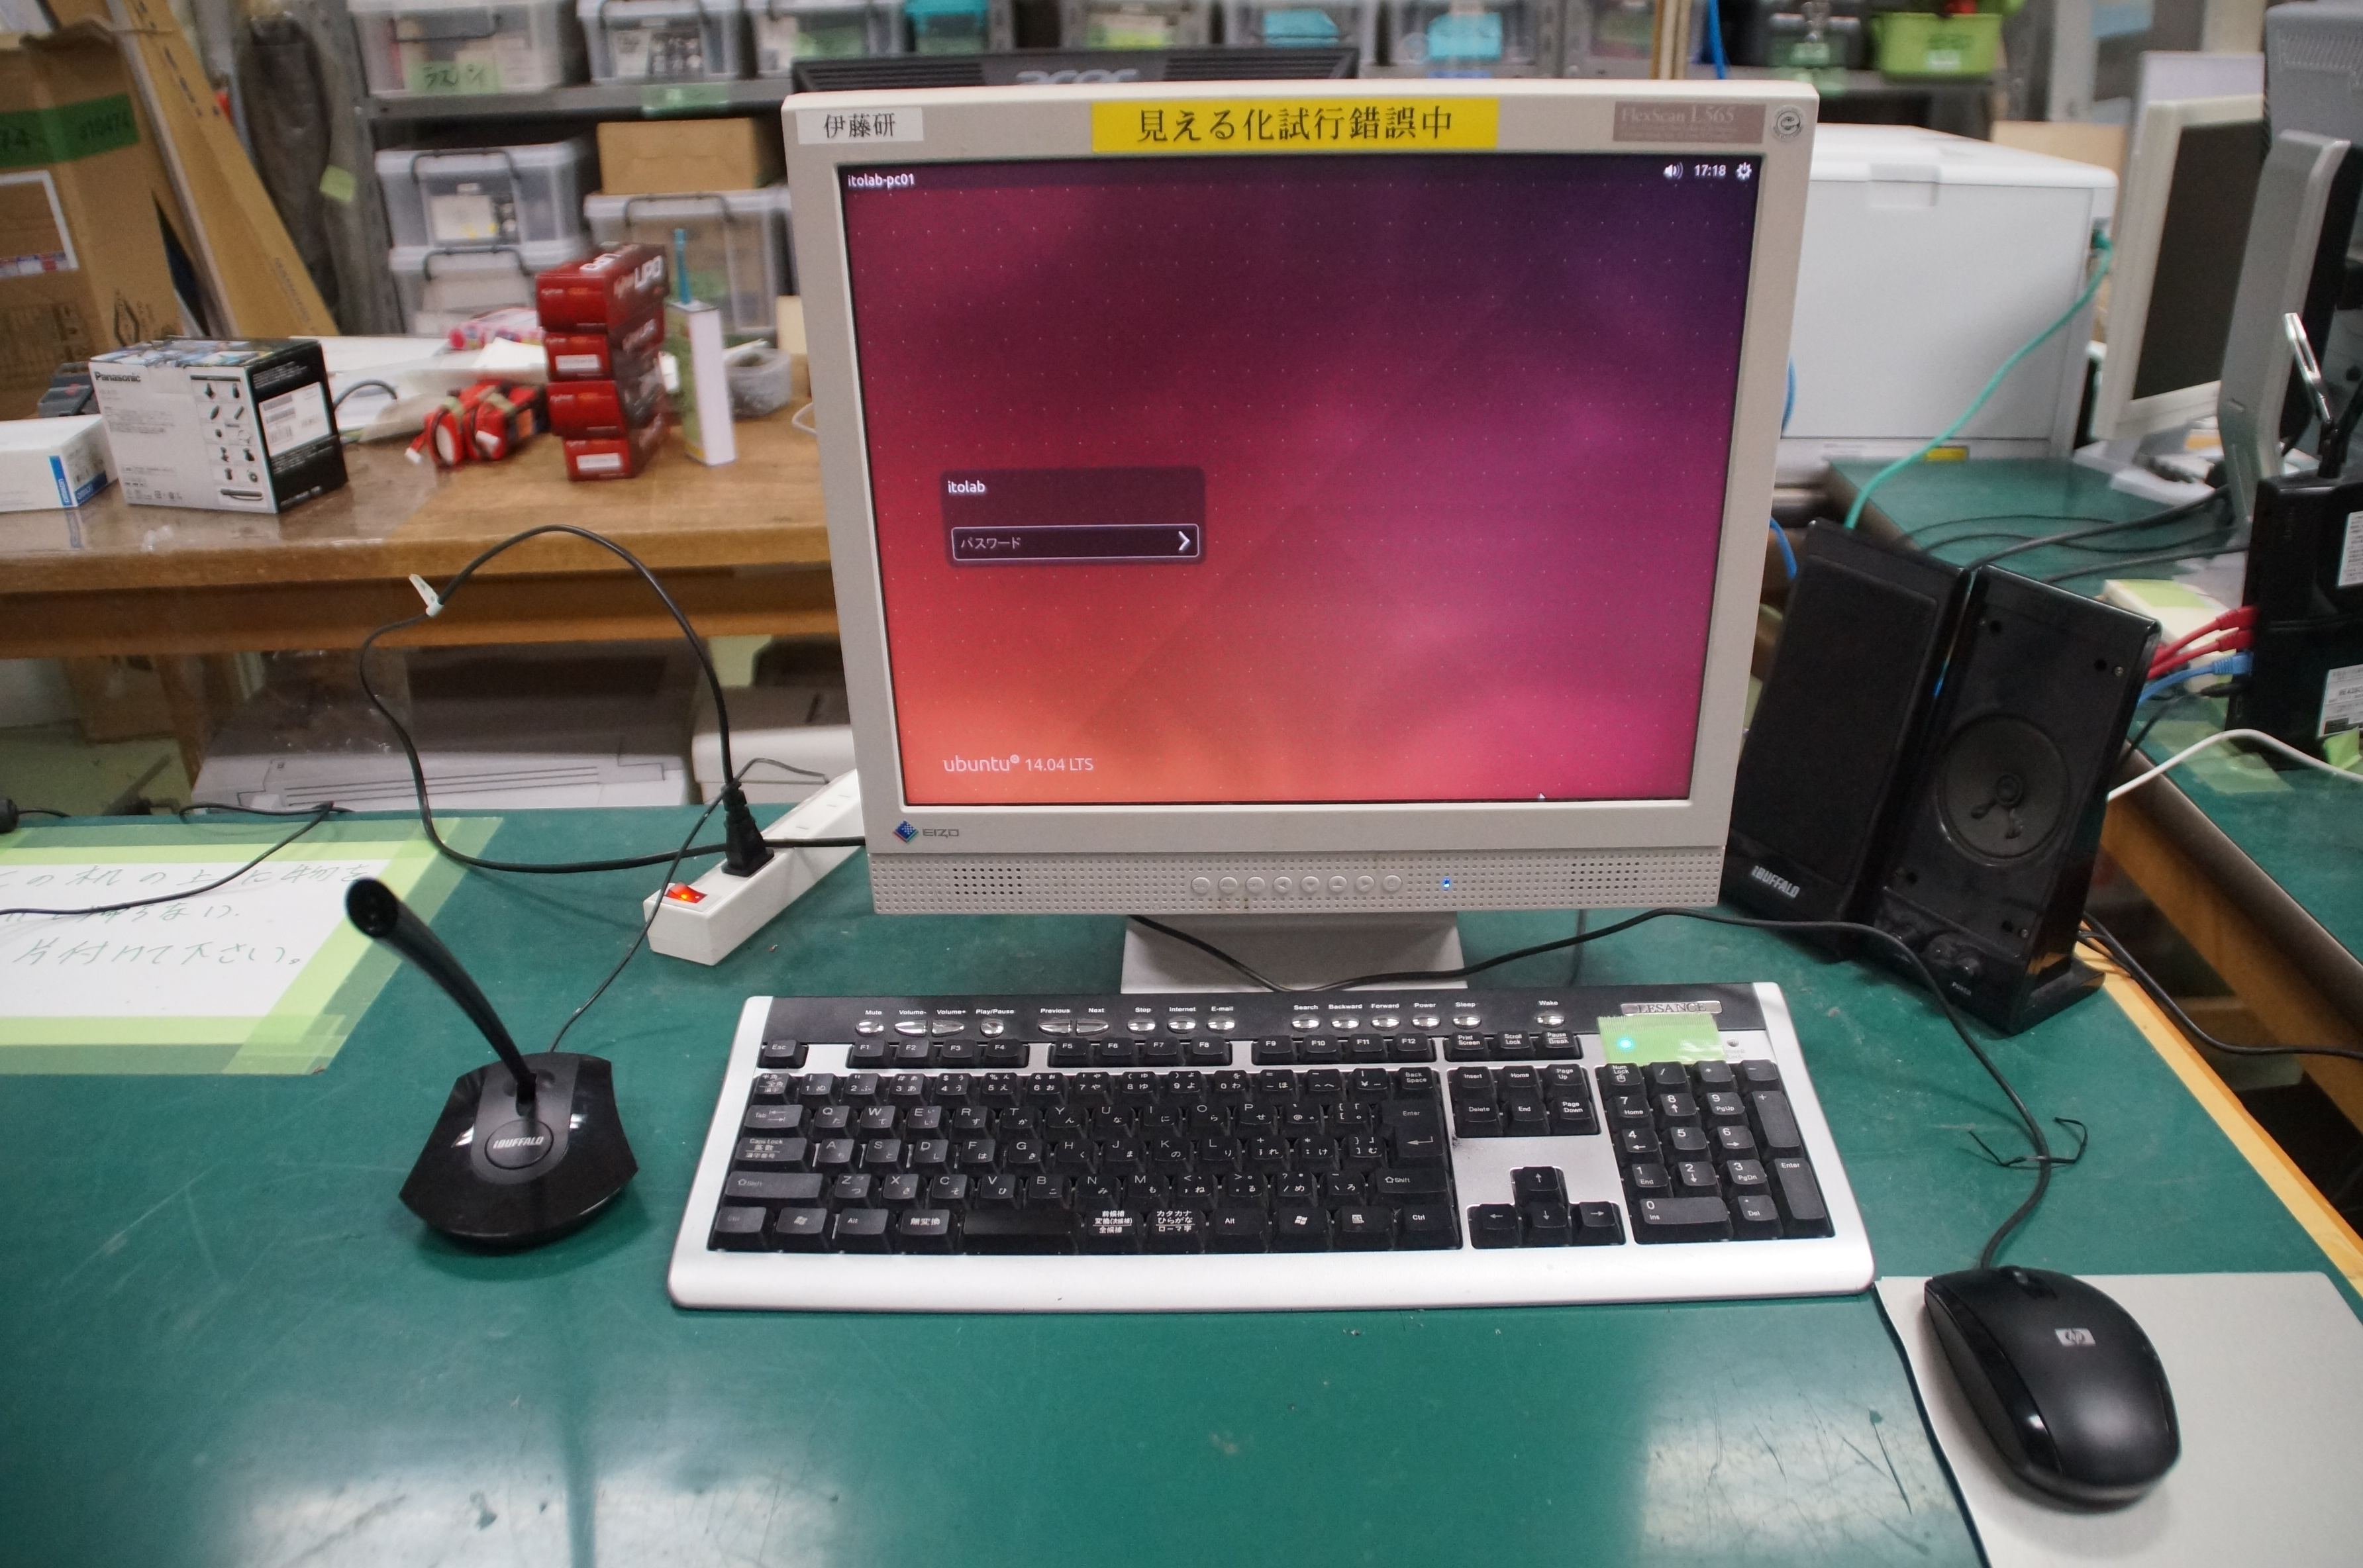
\includegraphics[width=120mm]{img/robo.JPG}
\caption{使用したシステム}
\label{fig:robot}
\end{center}
\end{figure}


\subsection{実験で使用するマイク}
本研究ではbuffalo製のマイク(BSHSM04BK)を使用した.その図を図\ref{fig:mic}に示す.


\begin{figure}[htbp]
\begin{center}
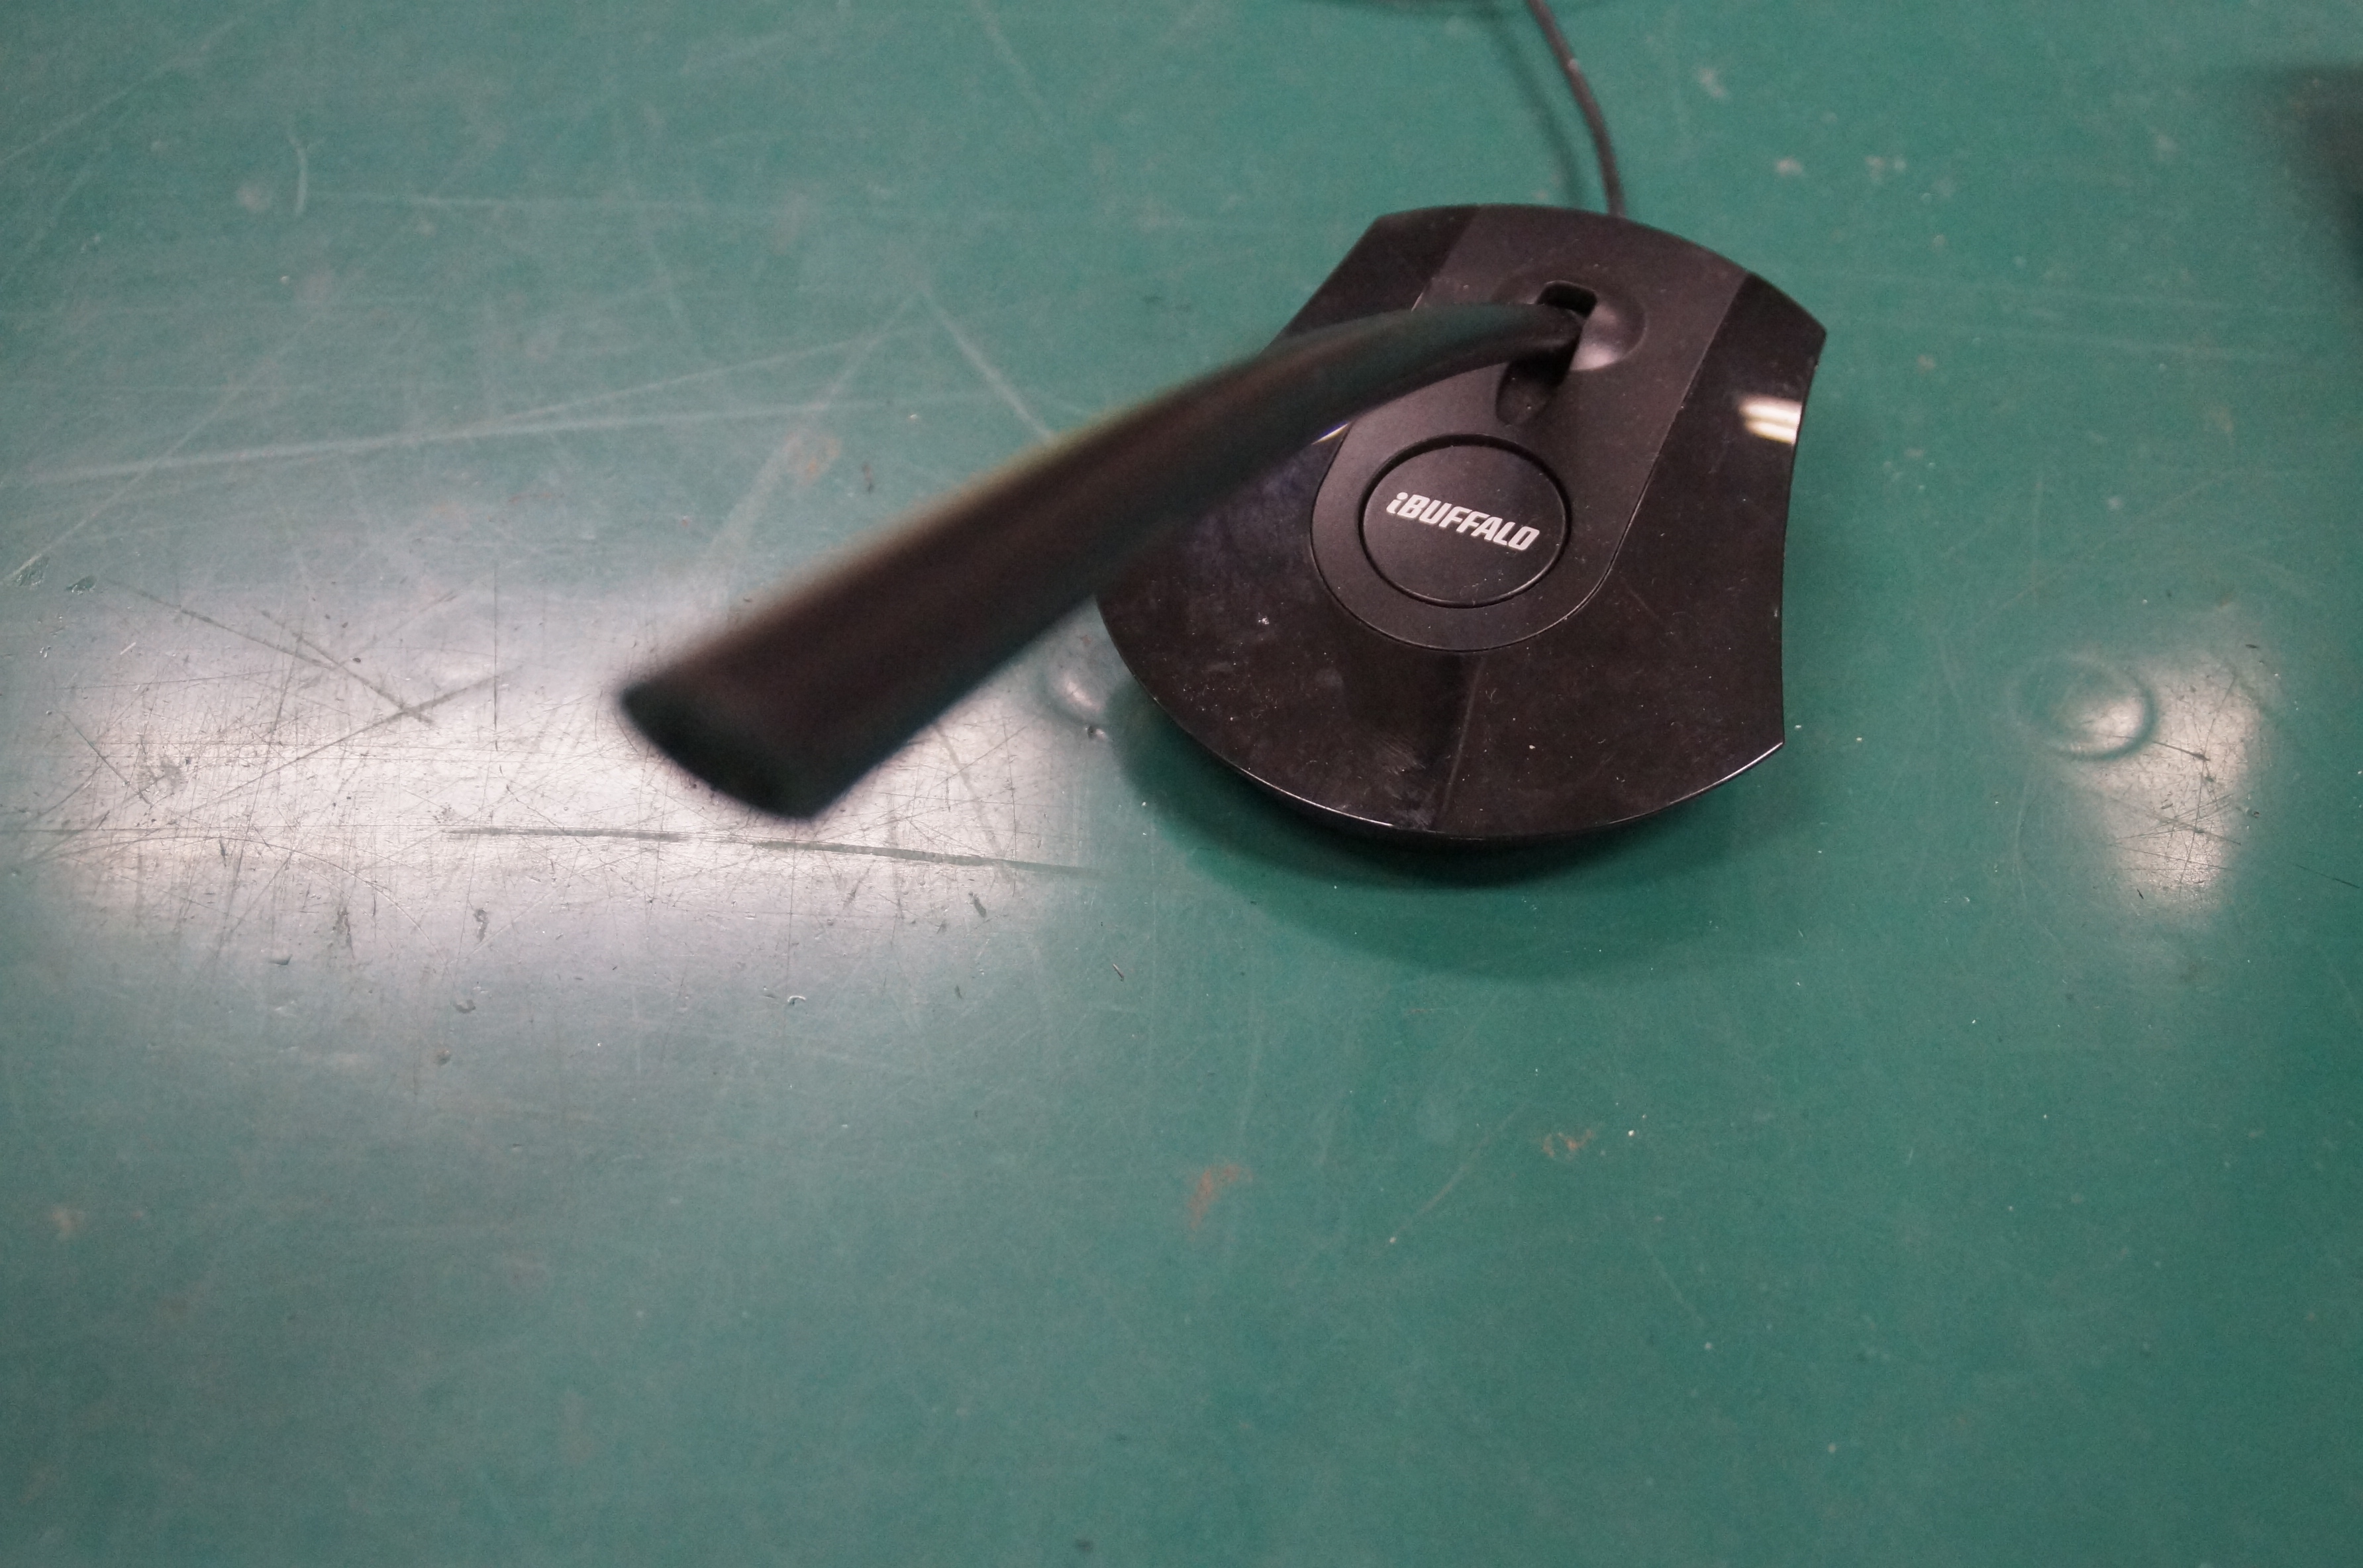
\includegraphics[width=120mm]{img/mic.JPG}
\caption{使用したマイク}
\label{fig:mic}
\end{center}
\end{figure}


\subsection{Julius}
Juliusは,音声認識システムの開発・研究のためのオープンソースの高性能な汎用大語彙連続音声認識エンジンである.数万語彙の連続音声認識を一般のPC上でほぼ実時間で実行できる.また,高い汎用性を持ち,発音辞書や言語モデル・音響モデルなどの音声認識の各モジュールを組み替えることで,様々な幅広い用途に応用できる.[2]Juliusはコマンド1つで起動させることができ,オプションでサーバモードで使用できるため,今回はサーバモードで起動し,クライアント側で認識した単語に対応した音声を発生させることを目指す.また本研究で使用したJuliusは最新版としてバージョン4.4.2が平成28年9月12日にGithubにて更新されている.しかし,研究を始めた時点でバージョン4.3.1が最新版だったためこれを継続して使用することとした.

\subsubsection{Juliusの仕組み}
Juliusの音声認識アルゴリズムは,ツリートレリス探索方式を基礎とするアルゴリズムである.全体は2パス構成となっており,2段階に分けて認識処理を行う.まず,第1パスでは入力全体に対して荒い認識処理を行い,有望な候補の集合をある程度絞り込む.このとき,簡便なモデルや近似計算を用いることで高速に処理を行う.第2パスでは詳細な認識処理を行うが,その際に第1パスの結果を参照しながら探索を行うことで,必要な部分にだけ精密な再計算を行って,最終的な最尤解を求める.[3]


\subsection{Open-JTalk}
Open-JTalkは,日本語テキストを音声に変換するシステムである.ここでは案内のために使用する音声の内容をWAVファイルとして保存するために使用する.「今回はあちらの席へどうぞ」,「こちらの席へどうぞ」の2つをWAVファイルとして保存した.


\chapter{音声認識実験}
\section{実験目的}
今回Juliusを使用して音声を認識させ,100回分の認識結果を集計し平均を取ることを目的とする.


\subsection{実験方法}
マイクを実装したパソコンを使用し,Juliusを端末より起動させる.Juliusを使用し,「禁煙です」,「喫煙です」,「吸います」,「吸いません」,「吸わないです」の認識を行う.このとき100回分の認識したときと認識しなかったときの結果を集計する.100回分の認識結果の平均を式\ref{eq:average}より算出する.

\begin{equation}
  x = a / 100
\end{equation}
\label{eq:average}


\subsection{実験結果}
\subsection{Juliusを用いて行った実験結果}
今回Juliusを用いて実験を行い,前節に示した式より算出した認識率は禁煙が99%,喫煙が100%,吸いますが100%,吸いませんが30%,吸わないですが100%という結果が得られた.また,マイクと被験者との距離を遠く取り,実験を行った.そのときの認識率は禁煙が90%,喫煙が86%,吸いますが43%,吸いませんが69%,吸わないですが71%だった.別条件での認識結果を表\ref{tab:nosmokerecogresult}に禁煙,表\ref{tab:smokrecogresult}に喫煙,表\ref{tab:yeahsmokrecogresult}に吸います,表\ref{tab:nonsmokrecogresult}に吸いません,表\ref{tab:neversmokrecogresult}に吸わないですの認識結果,\ref{tab:result}に認識結果一覧を示す.また,そのときのグラフを図\ref{fig:result}に示す.また,マイクとの距離を遠くして認識実験を行った結果, という結果が得られた.そのときの表を表\ref{tab:another-nosmokerecogresult},表\ref{tab:another-smokrecogresult},表\ref{tab:another-yeahsmokrecogresult},表\ref{tab:another-nonsmokrecogresult}表\ref{tab:another-neversmokrecogresult},に示す.グラフにしたものを\ref{fig:result2}に示す.


\begin{table}[htb]
\begin{center}
\caption{禁煙の認識結果}
\begin{tabular}{|c|c|c|c|c|c|c|c|}\hline
回数&禁煙です&回数&禁煙です&回数&禁煙です&回数&禁煙です\\\hline
1&○&26&○&51&○&76&○\\\hline
2&○&27&○&52&○&77&○\\\hline
3&○&28&○&53&○&78&○\\\hline
4&○&29&○&54&○&79&○\\\hline
5&○&30&○&55&○&80&○\\\hline
6&○&31&○&56&○&81&○\\\hline
7&○&32&○&57&○&82&○\\\hline
8&○&33&○&58&○&83&○\\\hline
9&○&34&○&59&○&84&○\\\hline
10&○&35&○&60&○&85&○\\\hline
11&○&36&○&61&○&86&○\\\hline
12&○&37&○&62&○&87&○\\\hline
13&○&38&○&63&○&88&○\\\hline
14&○&39&○&64&○&89&○\\\hline
15&○&40&○&65&○&90&○\\\hline
16&○&41&○&66&○&91&○\\\hline
17&○&42&○&67&○&92&○\\\hline
18&○&43&○&68&○&93&○\\\hline
19&○&44&○&69&○&94&○\\\hline
20&○&45&○&70&○&95&○\\\hline
21&○&46&○&71&○&96&○\\\hline
22&○&47&○&72&○&97&○\\\hline
23&○&48&○&73&○&98&○\\\hline
24&○&49&○&74&○&99&○\\\hline
25&○&50&○&75&○&100&○
\\\hline
\end{tabular}
\label{tab:nosmokerecogresult}
\end{center}
\end{table}


\begin{table}[htb]
\begin{center}
\caption{喫煙の認識結果}
\begin{tabular}{|c|c|c|c|c|c|c|c|}\hline
回数&喫煙です&回数&喫煙です&回数&喫煙です&回数&喫煙です\\\hline
1&○&26&○&51&○&76&○\\\hline
2&○&27&○&52&○&77&○\\\hline
3&○&28&○&53&○&78&○\\\hline
4&○&29&○&54&○&79&○\\\hline
5&○&30&○&55&○&80&○\\\hline
6&○&31&○&56&○&81&○\\\hline
7&○&32&○&57&○&82&○\\\hline
8&○&33&○&58&○&83&○\\\hline
9&○&34&○&59&○&84&○\\\hline
10&○&35&○&60&○&85&○\\\hline
11&○&36&○&61&○&86&○\\\hline
12&○&37&○&62&○&87&○\\\hline
13&○&38&○&63&○&88&○\\\hline
14&○&39&○&64&○&89&○\\\hline
15&○&40&○&65&○&90&○\\\hline
16&○&41&○&66&○&91&○\\\hline
17&○&42&○&67&○&92&○\\\hline
18&○&43&○&68&○&93&○\\\hline
19&○&44&○&69&○&94&○\\\hline
20&○&45&○&70&○&95&○\\\hline
21&○&46&○&71&○&96&○\\\hline
22&○&47&○&72&○&97&○\\\hline
23&○&48&○&73&○&98&○\\\hline
24&○&49&○&74&○&99&○\\\hline
25&○&50&○&75&○&100&○
\\\hline
\end{tabular}
\label{tab:smokrecogresult}
\end{center}
\end{table}


\begin{table}[htb]
\begin{center}
\caption{吸いますの認識結果}
\begin{tabular}{|c|c|c|c|c|c|c|c|}\hline
回数&吸います&回数&吸います&回数&吸います&回数&吸います\\\hline
1&○&26&○&51&○&76&○\\\hline
2&○&27&○&52&○&77&○\\\hline
3&○&28&○&53&○&78&○\\\hline
4&○&29&○&54&○&79&○\\\hline
5&○&30&○&55&○&80&○\\\hline
6&○&31&○&56&○&81&○\\\hline
7&○&32&○&57&○&82&○\\\hline
8&○&33&○&58&○&83&○\\\hline
9&○&34&○&59&○&84&○\\\hline
10&○&35&○&60&○&85&○\\\hline
11&○&36&○&61&○&86&○\\\hline
12&○&37&○&62&○&87&○\\\hline
13&○&38&○&63&○&88&○\\\hline
14&○&39&○&64&○&89&○\\\hline
15&○&40&○&65&○&90&○\\\hline
16&○&41&○&66&○&91&○\\\hline
17&○&42&○&67&○&92&○\\\hline
18&○&43&○&68&○&93&○\\\hline
19&○&44&○&69&○&94&○\\\hline
20&○&45&○&70&○&95&○\\\hline
21&○&46&○&71&○&96&○\\\hline
22&○&47&○&72&○&97&○\\\hline
23&○&48&○&73&○&98&○\\\hline
24&○&49&○&74&○&99&○\\\hline
25&○&50&○&75&○&100&○
\\\hline
\end{tabular}
\label{tab:yeahsmokrecogresult}
\end{center}
\end{table}


\begin{table}[htb]
\begin{center}
\caption{吸いませんの認識結果}
\begin{tabular}{|c|c|c|c|c|c|c|c|}\hline
回数&吸いません&回数&吸いません&回数&吸いません&回数&吸いません\\\hline
1&○&26&○&51&○&76&○\\\hline
2&○&27&○&52&○&77&○\\\hline
3&○&28&○&53&○&78&○\\\hline
4&○&29&○&54&○&79&○\\\hline
5&○&30&○&55&○&80&○\\\hline
6&○&31&○&56&○&81&○\\\hline
7&○&32&○&57&○&82&○\\\hline
8&○&33&○&58&○&83&○\\\hline
9&○&34&○&59&○&84&○\\\hline
10&○&35&○&60&○&85&○\\\hline
11&○&36&○&61&○&86&○\\\hline
12&○&37&○&62&○&87&○\\\hline
13&○&38&○&63&○&88&○\\\hline
14&○&39&○&64&○&89&○\\\hline
15&○&40&○&65&○&90&○\\\hline
16&○&41&○&66&○&91&○\\\hline
17&○&42&○&67&○&92&○\\\hline
18&○&43&○&68&○&93&○\\\hline
19&○&44&○&69&○&94&○\\\hline
20&○&45&○&70&○&95&○\\\hline
21&○&46&○&71&○&96&○\\\hline
22&○&47&○&72&○&97&○\\\hline
23&○&48&○&73&○&98&○\\\hline
24&○&49&○&74&○&99&○\\\hline
25&○&50&○&75&○&100&○
\\\hline
\end{tabular}
\label{tab:nonsmokrecogresult}
\end{center}
\end{table}


\begin{table}[htb]
\begin{center}
\caption{吸わないですの認識結果}
\begin{tabular}{|c|c|c|c|c|c|c|c|}\hline
回数&吸わないです&回数&吸わないです&回数&吸わないです&回数&吸わないです\\\hline
1&○&26&○&51&○&76&○\\\hline
2&○&27&○&52&○&77&○\\\hline
3&○&28&○&53&○&78&○\\\hline
4&○&29&○&54&○&79&○\\\hline
5&○&30&○&55&○&80&○\\\hline
6&○&31&○&56&○&81&○\\\hline
7&○&32&○&57&○&82&○\\\hline
8&○&33&○&58&○&83&○\\\hline
9&○&34&○&59&○&84&○\\\hline
10&○&35&○&60&○&85&○\\\hline
11&○&36&○&61&○&86&○\\\hline
12&○&37&○&62&○&87&○\\\hline
13&○&38&○&63&○&88&○\\\hline
14&○&39&○&64&○&89&○\\\hline
15&○&40&○&65&○&90&○\\\hline
16&○&41&○&66&○&91&○\\\hline
17&○&42&○&67&○&92&○\\\hline
18&○&43&○&68&○&93&○\\\hline
19&○&44&○&69&○&94&○\\\hline
20&○&45&○&70&○&95&○\\\hline
21&○&46&○&71&○&96&○\\\hline
22&○&47&○&72&○&97&○\\\hline
23&○&48&○&73&○&98&○\\\hline
24&○&49&○&74&○&99&○\\\hline
25&○&50&○&75&○&100&○
\\\hline
\end{tabular}
\label{tab:neversmokrecogresult}
\end{center}
\end{table}


\begin{table}[htb]
\begin{center}
\caption{認識結果一覧}
\begin{tabular}{|c|c|c|c|c|c|}\hline
単語&禁煙です&喫煙です&吸います&吸いません&吸わないです\\\hline
計&99&100&100&30&100\\\hline
平均&0.99&1&1&0.3&1
\\\hline
\end{tabular}
\label{tab:result}
\end{center}
\end{table}


\begin{figure}[htbp]
\begin{center}
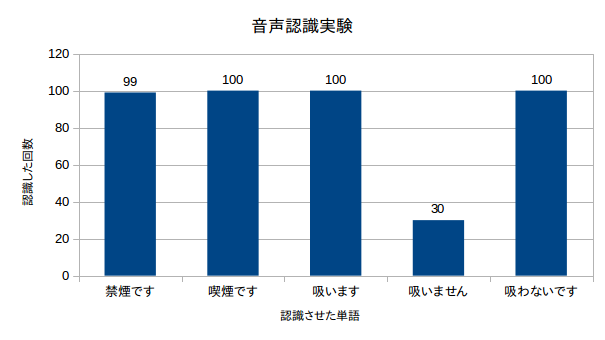
\includegraphics[width=150mm]{img/result.png}
\caption{認識結果グラフ}
\label{fig:result}
\end{center}
\end{figure}


\begin{table}[htb]
\begin{center}
\caption{別条件での禁煙の認識結果}
\begin{tabular}{|c|c|c|c|c|c|c|c|}\hline
回数&禁煙です&回数&禁煙です&回数&禁煙です&回数&禁煙です\\\hline
1&○&26&○&51&○&76&$\times$\\\hline
2&○&27&○&52&○&77&○\\\hline
3&$\times$&28&○&53&○&78&○\\\hline
4&$\times$&29&○&54&○&79&○\\\hline
5&○&30&○&55&○&80&○\\\hline
6&○&31&○&56&○&81&○\\\hline
7&○&32&○&57&○&82&○\\\hline
8&○&33&○&58&○&83&○\\\hline
9&○&34&○&59&$\times$&84&○\\\hline
10&○&35&○&60&○&85&$\times$\\\hline
11&○&36&○&61&○&86&$\times$\\\hline
12&○&37&○&62&○&87&$\times$\\\hline
13&○&38&○&63&○&88&○\\\hline
14&○&39&○&64&○&89&○\\\hline
15&○&40&○&65&○&90&$\times$\\\hline
16&○&41&○&66&○&91&○\\\hline
17&○&42&○&67&○&92&○\\\hline
18&○&43&○&68&○&93&○\\\hline
19&○&44&○&69&○&94&○\\\hline
20&○&45&○&70&○&95&○\\\hline
21&○&46&○&71&○&96&○\\\hline
22&○&47&○&72&○&97&○\\\hline
23&○&48&○&73&○&98&○\\\hline
24&○&49&○&74&○&99&○\\\hline
25&○&50&○&75&$\times$&100&$\times$
\\\hline
\end{tabular}
\label{tab:another-nosmokerecogresult}
\end{center}
\end{table}


\begin{table}[htb]
\begin{center}
\caption{別条件での喫煙の認識結果}
\begin{tabular}{|c|c|c|c|c|c|c|c|}\hline
回数&喫煙です&回数&喫煙です&回数&喫煙です&回数&喫煙です\\\hline
1&○&26&○&51&$\times$&76&○\\\hline
2&○&27&○&52&$\times$&77&○\\\hline
3&○&28&○&53&$\times$&78&○\\\hline
4&○&29&○&54&$\times$&79&○\\\hline
5&○&30&○&55&○&80&○\\\hline
6&○&31&○&56&○&81&○\\\hline
7&○&32&○&57&○&82&○\\\hline
8&○&33&$\times$&58&○&83&○\\\hline
9&○&34&$\times$&59&$\times$&84&○\\\hline
10&○&35&○&60&○&85&○\\\hline
11&○&36&○&61&○&86&○\\\hline
12&○&37&○&62&○&87&○\\\hline
13&○&38&○&63&○&88&○\\\hline
14&○&39&$\times$&64&○&89&○\\\hline
15&○&40&○&65&○&90&○\\\hline
16&○&41&○&66&○&91&○\\\hline
17&○&42&○&67&○&92&○\\\hline
18&○&43&○&68&○&93&○\\\hline
19&○&44&○&69&○&94&○\\\hline
20&○&45&○&70&○&95&○\\\hline
21&$\times$&46&○&71&○&96&○\\\hline
22&○&47&○&72&○&97&$\times$\\\hline
23&○&48&○&73&○&98&○\\\hline
24&○&49&$\times$&74&○&99&$\times$\\\hline
25&○&50&$\times$&75&○&100&$\times$
\\\hline
\end{tabular}
\label{tab:another-smokrecogresult}
\end{center}
\end{table}


\begin{table}[htb]
\begin{center}
\caption{別条件での吸いますの認識結果}
\begin{tabular}{|c|c|c|c|c|c|c|c|}\hline
回数&吸います&回数&吸います&回数&吸います&回数&吸います\\\hline
1&$\times$&26&$\times$&51&$\times$&76&$\times$\\\hline
2&○&27&○&52&○&77&$\times$\\\hline
3&$\times$&28&○&53&$\times$&78&○\\\hline
4&$\times$&29&○&54&$\times$&79&○\\\hline
5&$\times$&30&$\times$&55&$\times$&80&○\\\hline
6&$\times$&31&○&56&$\times$&81&○\\\hline
7&$\times$&32&$\times$&57&$\times$&82&○\\\hline
8&$\times$&33&○&58&○&83&○\\\hline
9&○&34&$\times$&59&$\times$&84&○\\\hline
10&$\times$&35&○&60&$\times$&85&○\\\hline
11&○&36&$\times$&61&$\times$&86&○\\\hline
12&○&37&$\times$&62&○&87&○\\\hline
13&$\times$&38&○&63&$\times$&88&○\\\hline
14&$\times$&39&○&64&$\times$&89&○\\\hline
15&○&40&○&65&$\times$&90&$\times$\\\hline
16&$\times$&41&○&66&$\times$&91&$\times$\\\hline
17&$\times$&42&○&67&$\times$&92&$\times$\\\hline
18&○&43&$\times$&68&$\times$&93&$\times$\\\hline
19&○&44&$\times$&69&○&94&$\times$\\\hline
20&○&45&$\times$&70&$\times$&95&$\times$\\\hline
21&$\times$&46&○&71&○&96&$\times$\\\hline
22&○&47&$\times$&72&$\times$&97&$\times$\\\hline
23&○&48&$\times$&73&○&98&$\times$\\\hline
24&$\times$&49&$\times$&74&$\times$&99&○\\\hline
25&○&50&$\times$&75&$\times$&100&○
\\\hline
\end{tabular}
\label{tab:another-yeahsmokrecogresult}
\end{center}
\end{table}


\begin{table}[htb]
\begin{center}
\caption{別条件での吸いませんの認識結果}
\begin{tabular}{|c|c|c|c|c|c|c|c|}\hline
回数&吸いません&回数&吸いません&回数&吸いません&回数&吸いません\\\hline
1&○&26&○&51&○&76&$\times$\\\hline
2&○&27&○&52&$\times$&77&○\\\hline
3&○&28&○&53&○&78&$\times$\\\hline
4&○&29&○&54&○&79&○\\\hline
5&○&30&○&55&○&80&$\times$\\\hline
6&○&31&○&56&$\times$&81&$\times$\\\hline
7&$\times$&32&○&57&○&82&$\times$\\\hline
8&○&33&○&58&$\times$&83&○\\\hline
9&○&34&○&59&○&84&$\times$\\\hline
10&○&35&○&60&○&85&$\times$\\\hline
11&○&36&○&61&$\times$&86&○\\\hline
12&○&37&○&62&○&87&○\\\hline
13&○&38&$\times$&63&$\times$&88&○\\\hline
14&○&39&○&64&○&89&○\\\hline
15&○&40&$\times$&65&○&90&○\\\hline
16&$\times$&41&$\times$&66&○&91&○\\\hline
17&$\times$&42&○&67&○&92&$\times$\\\hline
18&○&43&$\times$&68&$\times$&93&○\\\hline
19&○&44&$\times$&69&○&94&○\\\hline
20&○&45&○&7$\times$&○&95&○\\\hline
21&○&46&$\times$&71&$\times$&96&○\\\hline
22&$\times$&47&○&72&$\times$&97&○\\\hline
23&○&48&○&73&$\times$&98&○\\\hline
24&$\times$&49&○&74&$\times$&99&○\\\hline
25&$\times$&50&○&75&$\times$&100&○
\\\hline
\end{tabular}
\label{tab:another-nonsmokrecogresult}
\end{center}
\end{table}


\begin{table}[htb]
\begin{center}
\caption{別条件での吸わないですの認識結果}
\begin{tabular}{|c|c|c|c|c|c|c|c|}\hline
回数&吸わないです&回数&吸わないです&回数&吸わないです&回数&吸わないです\\\hline
1&○&26&○&51&○&76&$\times$\\\hline
2&○&27&○&52&$\times$&77&○\\\hline
3&○&28&○&53&$\times$&78&$\times$\\\hline
4&○&29&○&54&$\times$&79&○\\\hline
5&○&30&○&55&$\times$&80&○\\\hline
6&○&31&○&56&○&81&○\\\hline
7&○&32&○&57&○&82&○\\\hline
8&○&33&○&58&$\times$&83&○\\\hline
9&○&34&○&59&○&84&○\\\hline
10&○&35&○&60&○&85&$\times$\\\hline
11&○&36&○&61&○&86&$\times$\\\hline
12&○&37&○&62&○&87&$\times$\\\hline
13&○&38&○&63&$\times$&88&$\times$\\\hline
14&○&39&○&64&$\times$&89&$\times$\\\hline
15&○&40&○&65&○&90&$\times$\\\hline
16&○&41&○&66&○&91&$\times$\\\hline
17&○&42&○&67&○&92&○\\\hline
18&○&43&○&68&$\times$&93&○\\\hline
19&○&44&○&69&○&94&$\times$\\\hline
20&○&45&$\times$&70&○&95&○\\\hline
21&○&46&○&71&$\times$&96&$\times$\\\hline
22&○&47&$\times$&72&○&97&$\times$\\\hline
23&○&48&○&73&○&98&$\times$\\\hline
24&○&49&$\times$&74&$\times$&99&○\\\hline
25&○&50&$\times$&75&$\times$&100&$\times$
\\\hline
\end{tabular}
\label{tab:another-neversmokrecogresult}
\end{center}
\end{table}


\begin{table}[htb]
\begin{center}
\caption{別条件での認識結果一覧}
\begin{tabular}{|c|c|c|c|c|c|}\hline
単語&禁煙です&喫煙です&吸います&吸いません&吸わないです\\\hline
計&90&86&43&69&71\\\hline
平均&0.9&0.86&0.43&0.69&0.71
\\\hline
\end{tabular}
\label{tab:another-result}
\end{center}
\end{table}


\begin{figure}[htbp]
\begin{center}
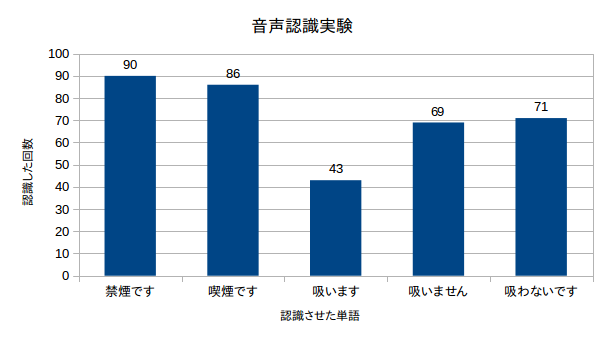
\includegraphics[width=150mm]{img/result2.png}
\caption{別条件での認識結果グラフ}
\label{fig:result2}
\end{center}
\end{figure}


\subsection{考察}
前述の音声認識実験での結果より認識率が99%,30%の単語が存在するがこれは「禁煙です」が「吸います」,「吸います」が「吸いません」と間違えたためである.また,「禁煙です」が「吸います」と誤認識をした原因は不明だが「吸います」と「吸いません」が極めて似ている単語であるため誤認識をしたのではないかと考えられる.また同じ被験者の方に協力していただき,マイクとの距離を変更して行った音声認識実験では「禁煙です」,「喫煙です」,「吸います」,「吸いません」,「吸わないです」の認識が成功した数が減少したのはinput rejected by short inputという認識不可を示す結果が出たためである.「吸いません」の音声認識実験を行った際に認識不可以外にも「喫煙です」と認識されることがあった.


\chapter{結言}
\section{本研究のまとめ}
音声を認識する接客ロボットのシステムを構築するにあたりJuliusを用いることで音声認識を行うことが可能となった.また,音声の認識結果より平均を算出することでJuliusの有用性を確かめることができた.今回は音声を作成するのみとなったが音声を認識した後に発声させる予定だった音声をWAVファイルとして作成し,保存することができた.これによって音声を認識した後に対応した音声を発声させることが出来る.


\section{今後の課題}
今後は研究者だけでなく研究者以外の人間を実験対象とし,認識率を算出する.また音声を認識したあとに認識した単語に対応した音声を発生させるプログラムをTCP/IPを介して組み合わせることにより,音声を認識し,認識した結果より対応した音声を発声させるためのシステムとして扱うことのできるシステムの確立がなされるのではないかと考える.また,このシステムを用いることで音声認識を用いた接客ロボットの開発を進めることができるのではないかと考える.


\begin{thebibliography}{9}
\bibitem{キー1} ディジタルアナログ信号処理のためのやさしいフーリエ変換 松尾 博 著 森北出版株式会社 1986年3月31日出版 P4-P5
\bibitem{キー2} Julius book 第7章 言語モデル・\url{https://julius.osdn.Jp/juliusbook/Ja/desc\_lm.html・2016/09/02閲覧}\\
\bibitem{キー3} Julius book 第8章 認識アルゴリズムとパラメータ \url{https://julius.osdn.jp/juliusbook/ja/desc_search.html#id2538692}・2017/01/20閲覧\\
\end{thebibliography}

\chapter*{謝辞}
\addcontentsline{toc}{chapter}{謝辞}
本論文作成にあたりテーマの決定,研究の考え方,方法のまとめ方など全てにおいて長期にわたって厳しくも熱意のあるご指導,ご鞭撻していただいた,伊藤恒平教授に厚く御礼申し上げます.


特に分析においても論文の書き方においても論文を何度も読んでいただき,指導していただいた伊藤恒平教授に大変ご苦労をかけてしまいましたことにも心よりお詫び申し上げたいです.


また音声認識実験に協力していただいた寺山森也君に厚く御礼申し上げます.


その他,助けていただいた多くの皆様に心から感謝しております.ありがとうございました.


\end{document}
